\documentclass[tikz]{standalone}

\colorlet{FilledSurface}{blue!20}
\colorlet{FilledSurfaceGroupOne}{blue!20}
\colorlet{FilledSurfaceGroupTwo}{red!20}
\colorlet{FilledSurfaceGroupThree}{green!20}
\colorlet{FilledSurfaceGroupFour}{magenta!20}
\colorlet{FormulaBackground}{green!10}
\colorlet{FormulaFrame}{green}


\usetikzlibrary{calc, angles}

\begin{document}
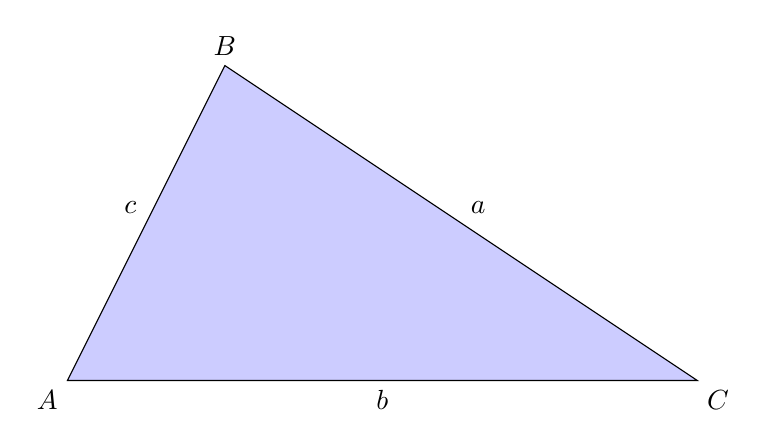
\begin{tikzpicture}

\coordinate (A) at (0,0);
\coordinate (B) at (2,4);
\coordinate (C) at (8,0);

\draw [fill=FilledSurfaceGroupOne] (A) node [below left]{$A$}
      -- node [above left] {$c$} (B) node [above]{$B$}
      -- node [above right] {$a$} (C) node [below right]{$C$}
      -- node [below] {$b$} cycle;

\end{tikzpicture}
\end{document}

